%%%%%%%%%%%%%%%%%%%%%%%%%%%%%%%%%%%%%%%%%%%%%%%%%%%%%%%%%%%%%%%%%%%
% Background
% Team:
% Wolverine
% Members: 
% Eric Lee, Jacky Wu, Karthick Mani, 
% Eric Chang, Dexter Chen, Peter Chen
% Relative files:
% Team_Wolverine.tex, Team_Wolverine_Compile.tex, Library.bib, WolverineChart.png
% Note:    
% Do not compile this file compile Main.tex to get the pdf file instead.
%%%%%%%%%%%%%%%%%%%%%%%%%%%%%%%%%%%%%%%%%%%%%%%%%%%%%%%%%%%%%%%%%%%
	
\subsection{Information retrieval of existing database}
Author: Eric Lee, Jacky Wu, Karthick Mani, Eric Chang, Dexter Chen, Yu-cheng Chen, Kenvin Lo

We live in the time where technologies evolve beyond our imagination. Due to the rapidly increasing amount of information, we can't rely on the use old fashion ways to store data. We need to create a database not only to store these data but also ease enough to access the data when needed.

A database management system (DBMS) is a computer  application that interacts with the user and other applications, the database itself  captures and analyze data. Well-known DBMSs include MySQL, PostgreSQL, Microsoft SQL Server, Oracle, Sybase and IBM DB2. And they can support different kinds of databases. This study includes numerous application and usage of such database as follows:

MySQL is the second rank relational database management system (RDBMS) and it is open-source. LAMP is an archetypal model of web service solution stacks, and its central component is MySQL. Web-based applications such as TYPO3 and MODx often use MySQL. MySQL is also applied in some famous website like Google, Facebook, and YouTube. It is able to be developed by the visual database design tool, MySQL Workbench.

Same as Relational database, object-oriented database management systems has developed since the 1970s. Db4o which was launched in 2004 represents an object-oriented database model. It provides an easy interface to work with object-oriented programming languages. And it also includes various object oriented-programming language. For this reason, the programmer can work in one environment persistently.

Finally, we’d like to introduce a DBMS, Neo4j. Neo4j is a graph database management system. It’s one of the most popular GDBMS, and it ranks 20 in the popularity of DBMS. Unlike other databases, relationships take first priority in graph databases. Also, the model is simpler and expressive than those of relational databases, such as NOSQL databases. Neo4j is widely used by organizations and has 1,000,000+ downloads. Because Neo4j is easy to learn and to use, it is for more easier for beginners to get used to the structure of graph databases. This study also introduced three kinds of DBMS, and the fallowing paragraph contains brief information about each kind of DBMS.

\paragraph{1. Object-oriented database}
An object-oriented database (OODBMS) is one of its  kind, a  database management     system.\cite{WiKiauthor2013} The information in the database is represented as objects as used in object-oriented programming.

Because of the tighter integration with the object-oriented language, the program is easier to maintain consistency with the same representation in both OODBMS and programming language.

Although relational databases which are table-oriented might be similar to object-oriented databases, But they are actually different. The object-oriented database supports objects, classes, and inheritance in database schemas and query language.
There are many advantages for OODBMS compared to the relational database management system(RODBMS) such as the performance, flexibility, and development cost.

And OODBMS also have some disadvantages, the \cite{Systems2010} have mention 3 disadvantage for OODBMS. First, because the usage is forced to be similar to an object-oriented language. This makes maintaining and evolving is  difficult. Second, the technique for store complex type of information takes additional computational resources. Third, lack of a standard data model leads to design errors and inconsistencies.


\paragraph{2. Relational database}
A relational database is the most popular database used in the world. They can organize data into one or more tables of columns and rows, with a unique key identifying each row. Rows are also called records or tuples. Generally, each table represents one "entity type" (such as customer or product). The rows represent instances of that type of entity (such as "Lee" or "iPhone 6") and the columns representing values attributed to that instance (such as address or price).

Because of the method of the organization of data, the relational database is much easier to understand and is flexible for you to manipulate the data. Besides SQL is easy in the relational database approach. For data organized in other structure, the query language either becomes complex or extremely limited in its capabilities. However, once the attributes of data become more and more, you'll need a large amount of table to store your information. Therefore, the performance of relational database will decrease obviously


\paragraph{3. Graph database}
A graphical database uses graph structures for semantic queries with nodes,  edges, and properties to represent and store data. Most graph databases are NoSQL in nature and store their data in a key-value store or document-oriented database. Graph databases are a powerful tool for graph-like queries, for example computing the shortest path between two nodes in the graph. Other graph-like queries can be performed over a graph database in a natural way.

When Compare to relational databases, there are several advantages. A graph database is often faster for associative data set and map more directly to the structure of object-oriented applications. They can scale more naturally to large data sets as they do not typically require expensive join operations. As they depend less on a rigid schema, they are more suitable to manage ad hoc and changing data with an evolving schema.

And graph database also comes with some disadvantages, the relational database is typically faster at performing the same operation on large numbers of data elements. AllegroGraph is one of the fine example for graph database: . 


According to many database websites and discussion thread, there are several methods to store a binary data with a database. The two main directions are store in the database and store out of the database. I will always be suggested not to store binary data in the database if the binary is large. That will cause significant performance decrease and additional storage space. And another way is to store binary data in the file system, and record the path in the database, that will not cause performance decrease when large binary data. But the binary data cannot automatically distribute with the database. Even the PDF document will cost some performance issues even though PDF file is small in size . And our system has no requirement to automatic distribute.  We suggest sorting  the PDF document is storing in the file system.

With the knowledge we gained  through this study will be utilised  to create a data base for open access full-text articles. The relational data base was decided as the structure in this study due to this structure has several advantages with which others cannot compare. For example, the relational database is so easy to learn that can make all participants know how to use that easier.secondly considering the availability of resources on the Internet which will help us accomplish the task much easier. However, authors believe, combining with others attractive and useful designs such as web crawler, user interface and so on, can be utilised to build a good data base  to  storethe full-text file like PDF.\\\\\\

%\begin{figure*}[h!]
\begin{wrapfigure}{i}{\textwidth}{WolverineChart}
	\begin{center}
		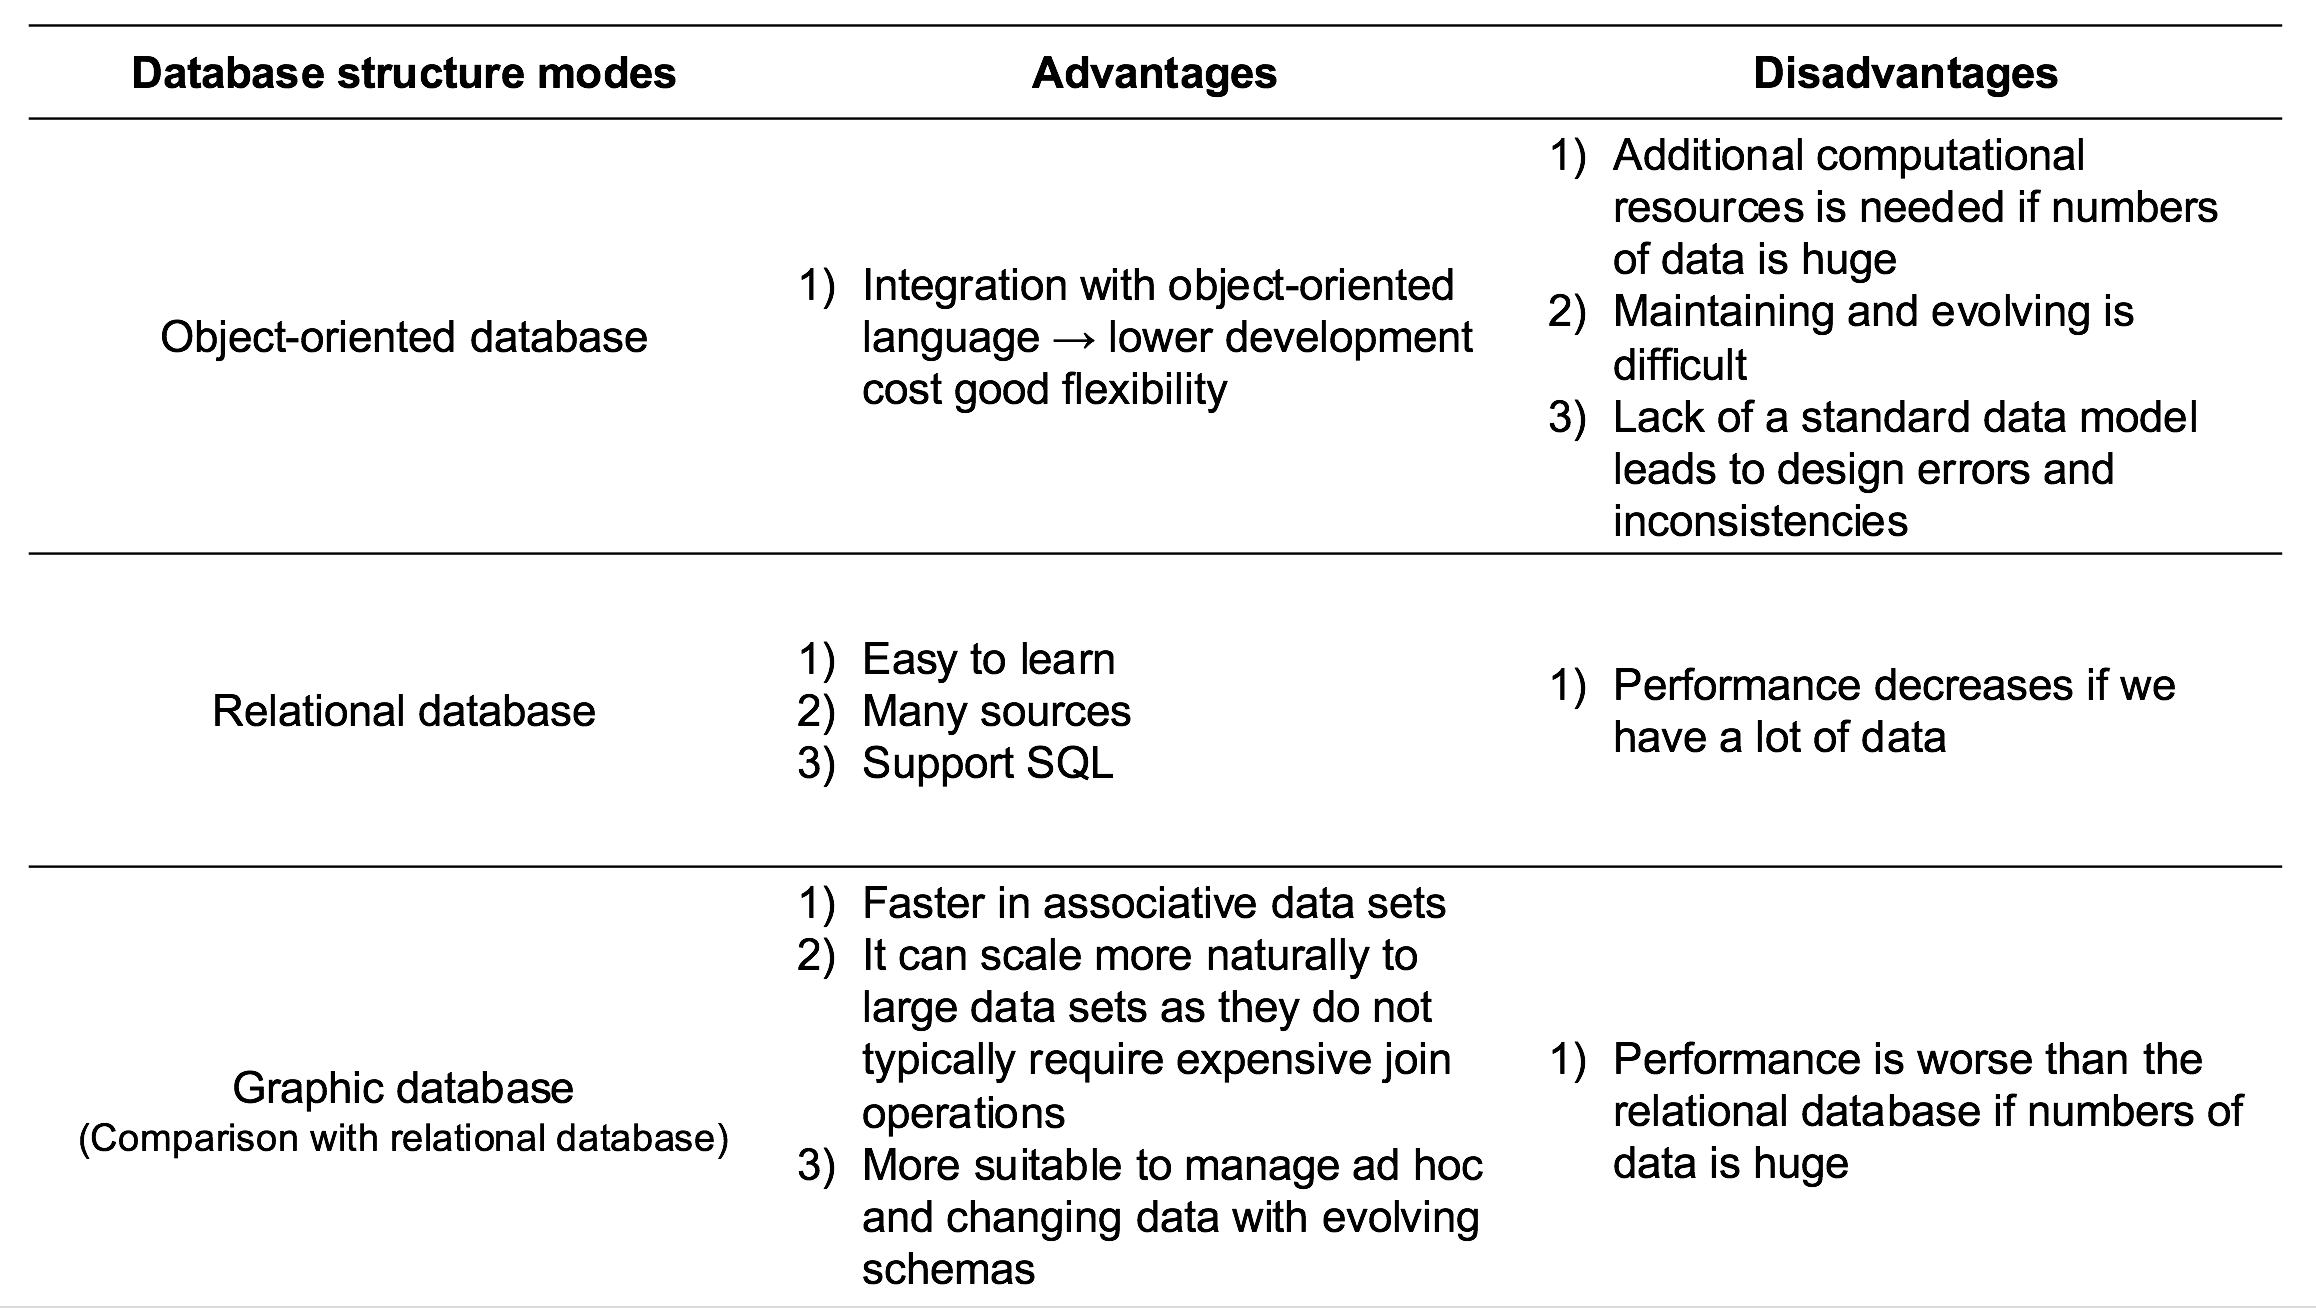
\includegraphics[width=0.8\textwidth]{WolverineChart2}
	\end{center}
	\caption{Database structure modes}
\end{wrapfigure}
%\end{figure*}
\clearpage
